%!TEX root=../main.tex

Neural networks have transformed machine learning.
Despite their success, little is known about
the global optima for typical non-convex training problems,
the solution path of regularized networks, or how to prune networks
without degrading the model fit.
This is in stark contrast to generalized linear models with \( \ell_2 \)
or \( \ell_1 \) penalties;
for example, it is well-known that the lasso \citep{tibshirani1996regression}
has a piece-wise linear path~\citep{osborne2000new, efron2004least},
a polyhedral solution set~\citep{tibshirani2013unique}, and
admits efficient algorithms for computing
minimal solutions~\citep{tibshirani2013unique}.
In this paper, we close the gap by studying neural networks
through the lens of convex reformulations.

\begin{figure}[t]
	\centering
	%\hspace{-2em}%
	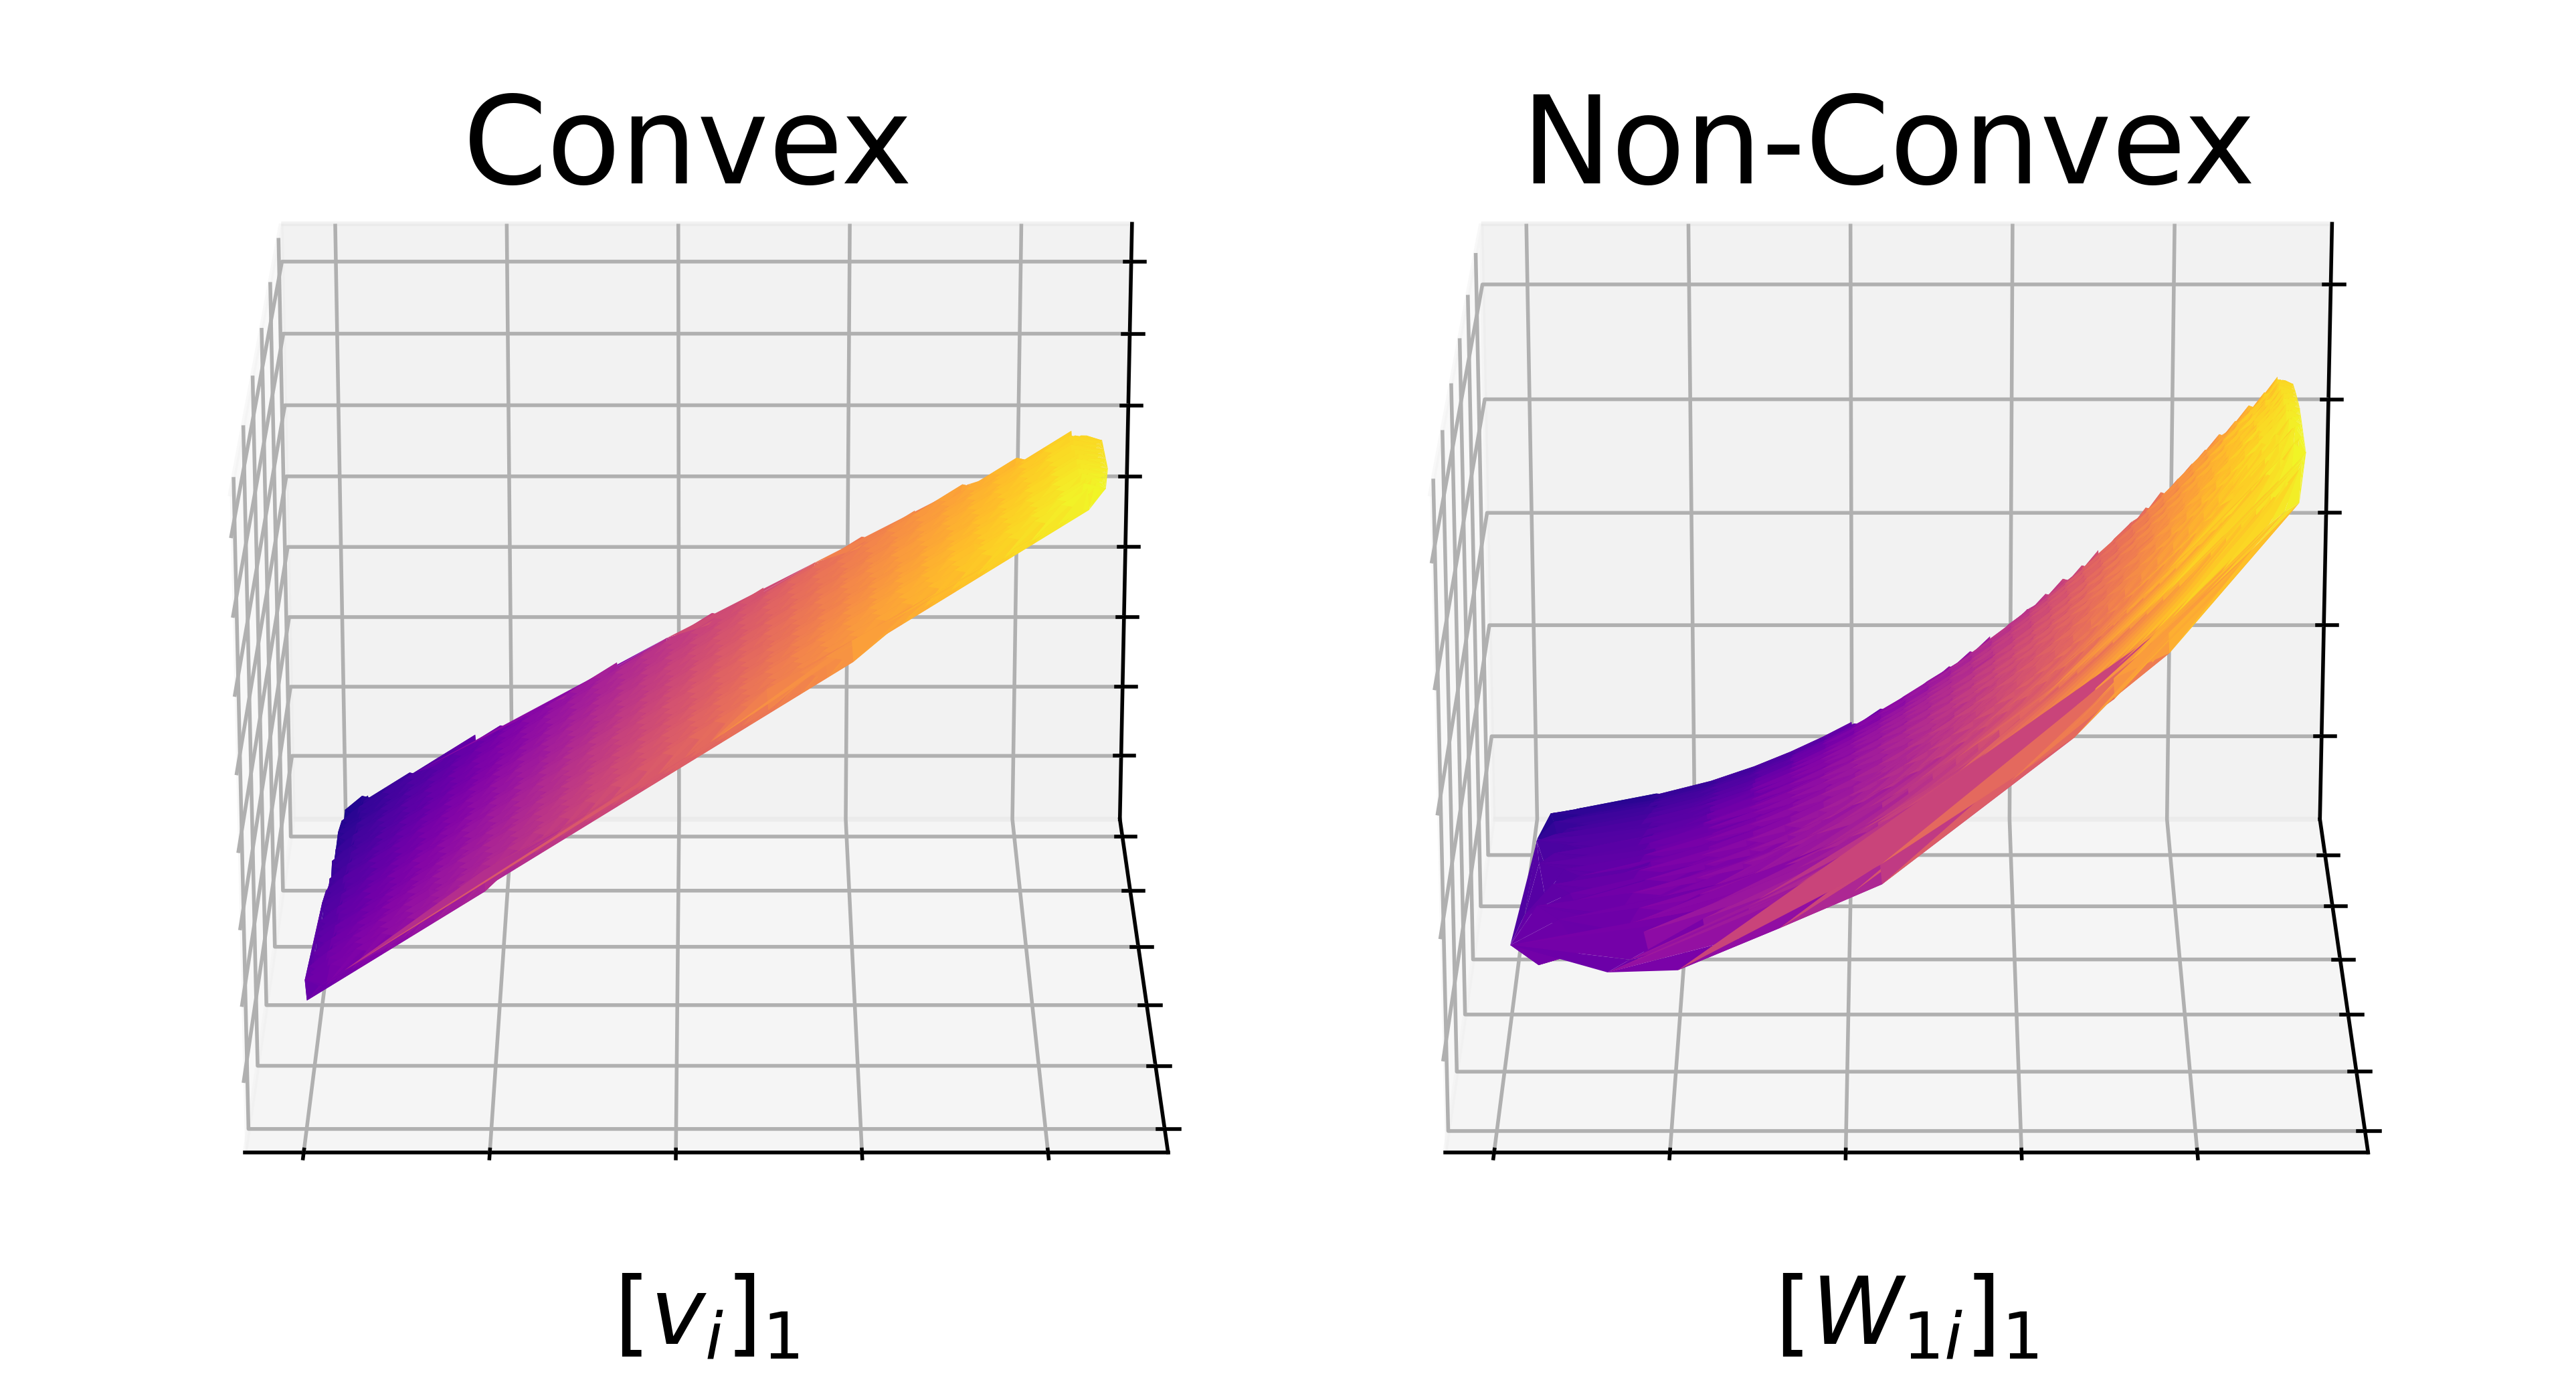
\includegraphics[width=0.5\textwidth]{figures/chapter_three/solution_sets_vis_270.png}
	\vspace{-3ex}
	\caption{Convex vs non-convex solution spaces for two-layer ReLU
		networks. We plot the first feature
		of three different neurons;
		the non-convex parameterization maps the compact polytope of
		solutions for the convex parameterization into a curved manifold.
	}
	\label{fig:solution-set}
\end{figure}

One of the main challenges of neural
networks is non-convexity.
For non-convex problems, stationarity of the training objective does not
imply optimality of the network weights and so, to the best of our knowledge,
no work has been able to derive an analytical expression for the optimal set.
Convex reformulations provide a solution by rewriting the non-convex
optimization problem as a convex program in a lifted parameter space
\citep{pilanci2020convexnn}.
We focus on the convex reformulation for two-layer networks with ReLU activation
functions and weight decay regularization.
The resulting problem is related to the group lasso \citep{yuan2006model}
and induces \emph{neuron sparsity} in the network.

Let \( Z \!\in\! \R^{n \times d} \) be a data matrix and \( y \!\in\! \R^n \) associated targets.
The prediction function for two-layer ReLU networks is
\begin{equation*}
	f_{W_1, w_2}(Z) = \sum_{i=1}^m \rbr{Z W_{1i}}_+ w_{2i},
\end{equation*}
where \( W_1 \in \R^{m \times d} \), \( w_2 \in \R^m \) are the weights of
the first and second layers, \( m \) is the number of hidden units,
and \( \rbr{\cdot}_+ = \max\cbr{\cdot, 0} \) is the ReLU activation.
Fitting \( f_{W_1, w_2} \) with convex loss \( L \)
and weight decay (\( \ell_2 \)) regularization leads to the
standard non-convex optimization problem:
\begin{equation}\label{eq:non-convex-relu-mlp}
	\min_{W_1, w_2} \! L\Big(f_{W_1, w_2}(Z), y \Big) + \frac{\lambda}{2} \underbrace{(\norm{W_{1}}_F^2 + \norm{w_{2}}_2^2)}_{R(W_1, w_2)}.\!
\end{equation}
The regularization path or \emph{solution function} of this training problem
is the mapping between the regularization parameter \( \lambda \) and the set of
optimal model weights,
\begin{equation}\label{eq:solution-function}
	\calO^*(\lambda) = \argmin_{W_1, w_2}  L\Big(f_{W_1, w_2}(Z), y \Big)
	+ \frac{\lambda}{2} R(W_1, w_2).\!
\end{equation}
In general, the optimal neural network is not unique and \( \calO^*(\lambda) \)
will be set valued.
Indeed, there are always at least \( m! \) solutions since any permutation of
the hidden units yields an identical model.
We call the solution to a ReLU training \emph{p-unique} when it is unique
up to splits and permutations.

We study \( \calO^* \) by re-writing
\cref{eq:non-convex-relu-mlp} as an instance of the
\emph{constrained group lasso} (CGL).
We make the following contributions by analyzing CGL:\

\begin{itemize}
	\item We derive an analytical expression for the solution set of two-layer
	      ReLU networks and criteria for solutions to be p-unique (unique up to
	      permutations/splits).
	      \vspace{-0.5ex}

	\item We extend this characterization to show that the set of
	      stationary points of a two-layer ReLU model is exactly
	      \vspace{-0.5ex}
	      \begin{equation}\label{eq:stationary-points}
		      \begin{aligned}
			      \calC_\lambda =
			       & \big\{
			      (W_1, \! w_2) : \tilde \calD \! \subseteq \! \calD_Z,
			      \, f_{W_1, w_2}(Z) \! = \! \hat y_{\tilde \calD},                              \\
			       & W_{1i} = (\sfrac{\alpha_{i}}{\lambda})^{\sfrac{1}{2}} v_i(\tilde \calD), \,
			      w_{2i} = \xi_i(\alpha_i \lambda)^{\sfrac{1}{2}},                               \\
			       & \alpha_i \geq 0, \, i \in [m] \setminus \calS_\lambda \implies \alpha_i = 0
			      \big\},
		      \end{aligned}
	      \end{equation}
	      where \( \tilde \calD \) is a set of sub-sampled activation patterns,
	      \( \hat y_{\tilde \calD} \) is the unique optimal model fit using
	      those patterns, and \( v_i(\tilde \calD) \) are uniquely given by optimal
	      parameters for the dual of the convex reformulation.
	      See \cref{fig:solution-set}.
	      \vspace{-0.5ex}

	\item We provide an optimal pruning algorithm that can be used to compute
	      minimal models --- the smallest-width neural networks which are optimal
	      for a given dataset and regularization parameter --- and an intuitive
	      extension for pruning beyond minimal models.
	      \vspace{-0.5ex}

	\item We prove that the regularization path of ReLU networks is discontinuous
	      in general and establish sufficient conditions for path to be
	      closed/continuous.
	      \vspace{-0.5ex}

	\item We give a simple algorithm for computing the unique ReLU network
	      corresponding to the min-norm model in the convex lifting and,
	      under additional constraint qualifications, develop differential
	      sensitivity
	      results for minimal ReLU networks.
	      \vspace{-0.5ex}
\end{itemize}
In many cases, we obtain strictly stronger results for gated ReLU networks
\citep{fiat2019decoupling},
which correspond directly to an unconstrained group lasso problem \citep{mishkin2022convex}.
In particular, we give new sufficient conditions for (i) the group lasso
to be unique, (ii) global continuity of the group lasso model fit, and (iii)
weak differentiability of the solution function for gated ReLU networks.

The paper is structured as follows: we cover related work in
\cref{sec:sol-fn-related-work}
and introduce notation in \cref{sec:notation}.
Then we provide details for convex reformulations of neural network
in \cref{sec:convex-reformulations}.
\cref{sec:cgl} analyzes CGL and
\cref{sec:specialization} interprets these results in the specific context of
two-layer ReLU networks.
\cref{sec:sol-fn-experiments} concludes with experiments.
